\section{Data Dashboards in Data Science}
A data dashboard is a tool that businesses use to track, analyse, and display data, usually to gain a better understanding of the overall health of the organization, a department, or even a specific process. Dashboards connect a variety of metrics, data sources, APIs, and services behind the scenes, assisting businesses in extracting relevant information from those sources and displaying it in user-friendly ways. Data dashboards, similar to a car's dashboard, organize and display important information at a glance to help you understand your company's most valuable data and find answers to critical questions. By linking dashboards to specific metrics or key performance indicators (KPIs), you gain valuable business intelligence as well as the ability to delve deeply into specific pieces of information to continuously monitor success. Dashboards, like those in cars, show how far you are along your journey and how long it may take to get to your destination.
A dashboard's ability to provide up-to-date information and context to help inform business decisions and empower employees is one of its most powerful features. A dashboard, for example, could be used by an IT team to help detect signs of a security breach. Alternatively, a company could incorporate the dashboard into an app or mobile device for first-line workers in the field, ensuring that they have access to the data they require at all times.
As for the digital twin case in this paper, our paper will be used visualize data, forecast data for Nth number of years, make predictions on a given date, find out the impacts of parameters in your dataset and find out how to optimize the production line or produce the best outcome for your plant/company.
Our parameters (dataset headers example .csv) can be described as a set of

\begin{center}
    $\{p_n | n=p_1,p_2,p_2,\dots\}$
\end{center}

where $p_n$ is a parameter.\\


Let’s say for example in a water plant our $p_1$ can be DateAndTime , $p_2$ = PropertyMeasurement , $p_3$ = SomeChemicalCompound … $p_n$ = our dataset parameters for a given index
We could sketch graphs on this data and predict values based on parameter behaviors. We can play around, modify some parameters and see what effect that makes on our plant. Our AI can also optimize the plant for the best-fine-tuned results for our plant. It can generate insights for us and tell us how we can improve the quality of our plant or object. Below are examples of the dashboard and the functionality it presents to us.

\begin{figure}
    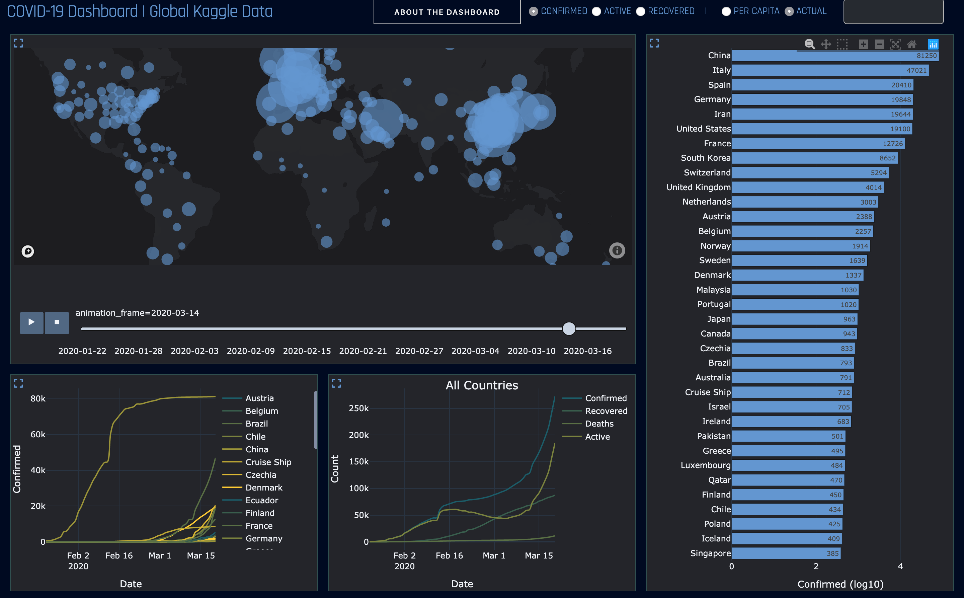
\includegraphics[width=\linewidth]{images/covid19dashboard.png}
    \caption{Example of a Covid-19 Dashboard just visualizing data with filters.}
    \label{fig:covid19dashboard}
\end{figure}

\begin{figure}
    \includegraphics[width=\linewidth]{images/stonkapppt1.png}
    \caption{Example of my application dashboard displaying JSE stocks for a given date interval and forecasting stocks for a given number of years https://stonks.adgstudios.co.za}
    \label{fig:stonkapppt1}
\end{figure}

\section{Machine Learning and Forecasting}
\subsection{Introduction to Machine Learning and Forecasting for building digital twins}

Machine learning and forecasting are important tools in the digital twin toolbox. It is the most important component of the digital twin; without these tools and knowledge, the digital twin would not exist. Artificial Intelligence includes the subcategory of Machine Learning. Machine Learning is used to find trends/equations created from Machine Learning models that best describe our data and will be used to make predictions based on input and output data.
Let me describe the above in simple mathematical equations. \\

Let’s take our old-school way of a simple function/formula to determine some sort of output. Let us say
\begin{equation}
    \{p_n | n=p_1,p_2,p_2,\dots\}
\end{equation}

where $p_n$ is our parameters.\\

\textbf{General Equations we are taught in life} \\


\begin{equation}
    f(p_n)= p_n+rules
\end{equation}

\begin{equation}
    f(\{p_n | n=p_1,p_2,p_2,…\}) = \{p_n | n=p_1,p_2,p_2,…\}+rules \\
\end{equation}


\begin{center}
In Layman’s Equation Terms \\ 
Input + rules = output \\ 
\end{center}

\begin{center}
    (Input is put through the rules returning some form of output)
\end{center}


\textbf{In normal programming} \\

\begin{equation}
    \{p_n | n=p_1,p_2,p_2,…\}  +rules= ? 
\end{equation}

\begin{center}
    In Layman’s Equation Terms \\ 
    Input + rules = output \\ 
\end{center}

\begin{center}
    Our question mark represents (output, but depends on input and/or rules)
\end{center}

\textbf{In Machine Learning} \\ 

Let us define some machine learning equation let’s say if we are using the KNN algorithm (more about that later in this paper)

\begin{equation}
f(p_n )= f_{KNN} (p_n) \\
\end{equation}

\begin{equation}
f(\{p_n | n=p_1,p_2,p_2,…\})= f_{KNN} (\{p_n | n=p_1,p_2,p_2,…\}) \\ 
\end{equation}

\begin{center}
In Layman’s Equation Terms \\ 
Input + ? = output \\
\end{center}


\begin{center}
In this case the ? means the rules (program makes rules based on input and
expected output)
\end{center}
 
I have built a Python Module to find the best parameters to trains your machine learning module.
It is called adgmlclass which is on PyPi and code is open source on my GitHub.
You could also set the rules to a generic machine learning algorithm, modify the algorithm with fine-tuned Machine Learning parameters. 

\begin{figure}[H]
    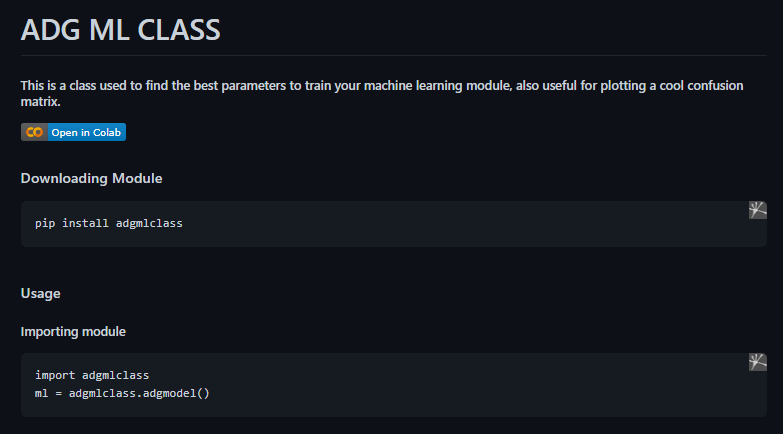
\includegraphics[width=\linewidth]{images/adgmlclassrepo.png}
    \caption{ADGMLCLASS : https://github.com/adgsenpai/adgmlclass}
    \label{fig:adgmlclass}
\end{figure}

\subsection{What is Machine Learning?}
Machine learning, also known as automatic learning, is a branch of science and a subcategory of artificial intelligence. It entails allowing algorithms to find "patterns" in data sets, i.e., recurring patterns. This information can take the form of numbers, words, images, statistics, and so on. Machine Learning can use anything that can be stored digitally as data.
Algorithms learn and improve their performance in performing a specific task by detecting patterns in this data.

\subsection{Which Mathematical Concepts Are Used in Machine Learning and Data Science?}
Statistics, Linear Algebra, Probability, and Calculus are the four key concepts that drive machine learning. While statistical concepts are at the heart of all models, calculus aids in the learning and optimization of those models.

\subsection{Importance of Machine Learning}
Machine learning is important because it allows businesses to see trends/predictions in customer behavior and business operational patterns while also assisting in the development of new products. Machine learning is at the heart of many of today's most successful businesses, including Facebook, Google, and Uber. In this paper, the importance of Machine Learning is that we are using it to predict and forecast data based on our input data which is the parameters to determine an output value on an output parameter.

\subsection{Machine Learning Types, Algorithms, and Usage}
\subsubsection{Types of Machine Learning:}
\textbf{Supervised Learning} \\ 
Supervised learning is a type of machine learning in which machine learning
from known datasets (set of training examples), and then predict the output.
A supervised learning agent needs to find out the function that matches a given sample set.
Supervised learning further can be classified into two categories of algorithms:
\begin{enumerate}
\item Classifications
\item Regression
\end{enumerate}

\textbf{Unsupervised Learning} \\ 
Unsupervised learning is associated with learning without supervision or 
training. In unsupervised learning, the algorithms are trained with data
which is neither labeled nor classified. In unsupervised learning,
the agent needs to learn from patterns without corresponding output values.
Unsupervised learning can be classified into two categories of algorithms:

\begin{enumerate}
\item Clustering
\item Association
\end{enumerate}


\textbf{Reinforcement Learning} \\ 
Reinforcement learning is a type of learning in which an AI agent is trained by giving some commands, and on each action, an agent gets a reward as feedback. Using these feedbacks, agent improves its performance. Reward feedback can be positive or negative which means on each good action, agent receives a positive reward while for wrong action, it gets a negative reward.
Reinforcement learning is of two types:
\begin{enumerate}
\item Positive Reinforcement learning
\item Negative Reinforcement learning
\end{enumerate}


\subsubsection{List of Common Machine Learning Algorithms}
% generate list
\begin{itemize}
\item \textbf{Linear Regression – (will explain the algorithm in paper)}
\item Logistic Regression
\item Decision Tree
\item SVM
\item Naive Bayes
\item \textbf{KNN – (will explain the algorithm in paper)}
\item K-Means
\item Random Forest
\item Dimensionality Reduction Algorithms
\item Gradient Boosting algorithms
\item Autoencoder
\item Convolutional Neural Network
\item Recurrent Neural Network
\item Support Vector Machine
\item Deep Learning
\end{itemize}

Deep learning is another complicated topic that I won't go into much detail about in this paper; instead, I'll give you some general information about it. Deep learning is a subset of a larger family of machine learning techniques based on representation learning and artificial neural networks. There are three types of learning: supervised, semi-supervised, and unsupervised. For image classification, object detection, image restoration, and image segmentation, deep learning has delivered superhuman accuracy—even handwritten digits can be recognized. Deep learning, which makes use of massive neural networks, is teaching machines to automate the tasks that human visual systems perform. Deep learning is a machine learning and artificial intelligence (AI) technique that mimics how humans acquire knowledge.

\begin{figure}[H]
    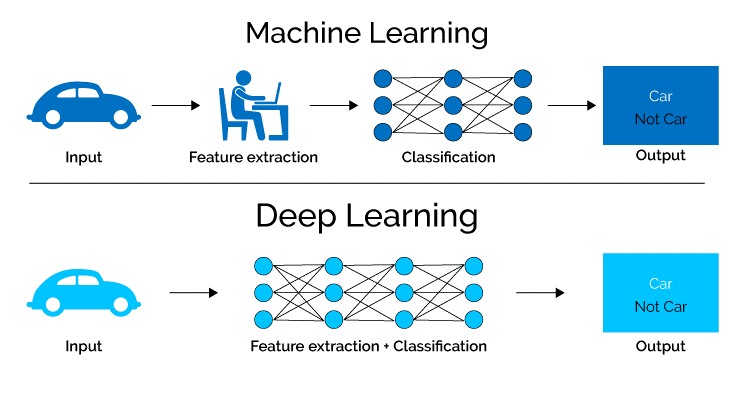
\includegraphics[width=\linewidth]{images/deeplearningdiagram.png}
    \caption{Deep Learning General Structure Diagram}
    \label{fig:deeplearningexplained}
\end{figure}

\subsection{Linear Regression}
\subsubsection{Introduction to Linear Regression}

A linear approach to modeling the relationship between a scalar response and one or more explanatory variables is known as linear regression in statistics. Simple linear regression is used when there is only one explanatory variable; multiple linear regression is used when there is more than one. 
Linear regression is a supervised machine-learning regression algorithm. \\
A typical linear regression equation that you learned in high school is in the form of
\begin{equation}
y = b_0 + b_1 x
\end{equation}

where $y$ is the response variable, $b_0$ is the intercept, and $b_1$ is the coefficient. \\

\begin{figure}[H]
    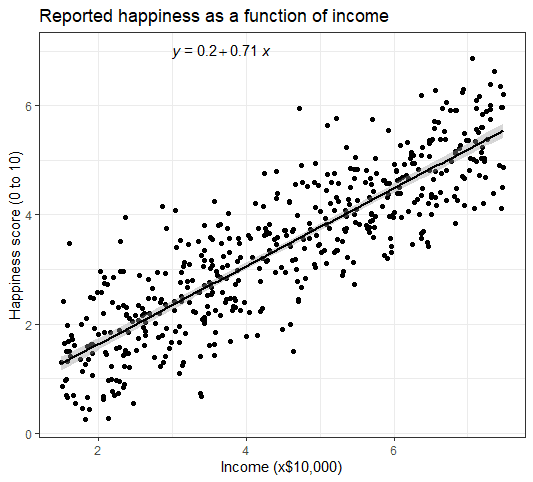
\includegraphics[width=\linewidth]{images/linearregeg.png}
    \caption{Linear Regression function of Reported Happiness by income values}
    \label{fig:linearregressionfunction}
\end{figure}

In this example, employees are interviewed and are asked to fill in the form below.
Rate your happiness in life from 

\begin{equation}
y \in \left\{0..10\right\} 
\end{equation}
 
We capture our data and represent it in a digital format or record it on a page.
The data scientist visualizes the data in a scatter graph. To make predictions on this data he calculates the regression equation which is 

\begin{equation}
y=0.2+0.71x 
\end{equation}

and plots the function on the scatter graph. If you look at the diagram above that is exactly what is being done to predict data. \\

\textbf{Simple Prediction and Flaw with Linear Regression} \\ 
Let us predict my happiness score based on this model. \\ 

where $x$ is the income in 10k \\
and $y$ is the happiness score.

\begin{equation}
    y=0.2+0.71(100)
\end{equation}

Our predicted score is \textbf{71.2}. That is not possible as the scale can only be $y \in \left\{0..10\right\}$
You can see that the model above is invalid and inaccurate. The training size is too small. We could get a better model if we use a larger population. The point I’m trying to make with Linear Regression is that you will get false alerts and reading based on the input data. I would also say emotions with people are not accounted for when working with Machine Learning models. For example, some people who are multi-millionaires are depressed with life. Some people with low income are happy in life they appreciate the simple things in life. Machine Learning does not account for emotion there is another aspect in AI that can help predict emotions and that is called Natural Language Processing. It works with text and speech. Deep learning powers that technology.\\

\textbf{Other types of Linear Regression} \\
What I showed you in the introduction was a \textbf{simple linear regression} equation which is 
\begin{equation}
y = b_0 + b_1 x
\end{equation}

where $y$ is the response variable, $b_0$ is the intercept, and $b_1$ is the coefficient. \\

A simple graph of that is 
\begin{figure}[H]
    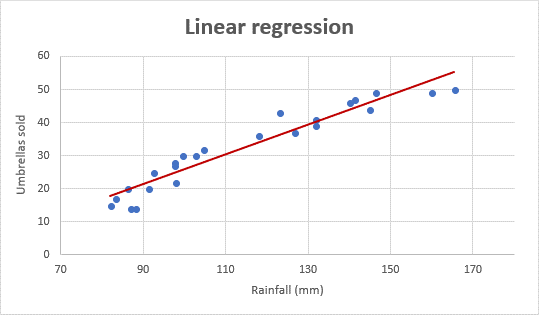
\includegraphics[width=\linewidth]{images/simplereg.png}
    \caption{Simple Linear Regression}
    \label{fig:simplelinearreg}
\end{figure}

The second type of linear regression is called \textbf{Multiple Linear Regression}
\begin{equation}
y = \beta_0 + \beta_1 x_1 + \beta_2 x_2^2 + \cdots + \beta_n x^n
\end{equation}
    
    where $y$ is the response variable, $\beta_0$ is the intercept, and $\beta_1$ is the coefficient for $x_1$, $\beta_2$ is the coefficient for $x_2^2$, and so on. \\


\begin{figure}[H]
    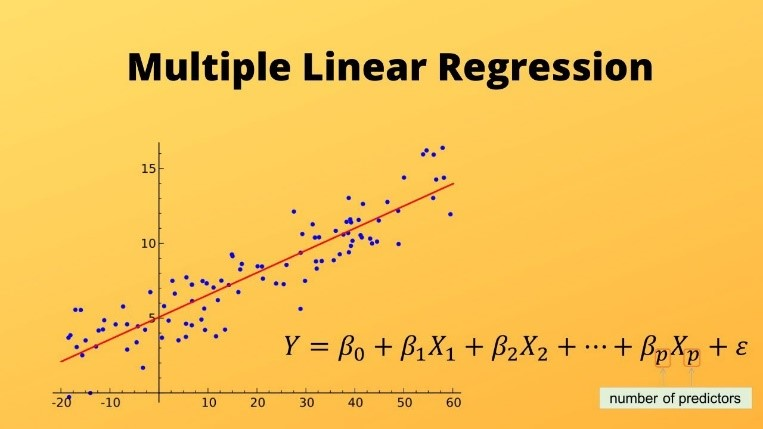
\includegraphics[width=\linewidth]{images/mlrgraph.jpg}
    \caption{Multiple Linear Regression}
    \label{fig:mlr}
\end{figure}


A graph for multiple linear regression looks similar to the simple linear regression above.

The last type of linear regression is called \textbf{Polynomial Linear Regression}
\begin{equation}
y = \beta_0 + \beta_1 x_1 + \beta_2 x_1^2 + \cdots + \beta_n x_1^n
\end{equation}
    
    where $y$ is the response variable, $\beta_0$ is the intercept, and $\beta_1$ is the coefficient for $x_1$, $\beta_2$ is the coefficient for $x_1^2$, and so on. \\
 
    \begin{figure}[H]
        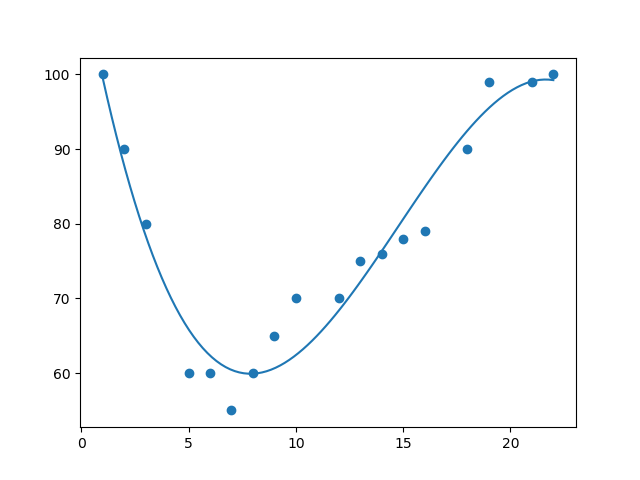
\includegraphics[width=\linewidth]{images/plr.png}
        \caption{Multiple Linear Regression}
        \label{fig:plr}
    \end{figure}
    
\subsection{K-Nearest Neighbors}
\subsubsection{Introduction to K-Nearest Neighbors}
K-nearest neighbors (k-NN) is a supervised machine learning algorithm that can be used to solve both classification and regression tasks.
Suppose there are two categories, i.e., Category A and Category B, and we have a new data point x1, so this data point will lie in which of these categories. To solve this type of problem, we need a K-NN algorithm. With the help of K-NN, we can easily identify the category or class of a particular dataset. \\ Consider the below diagram:

    \begin{figure}[H]
        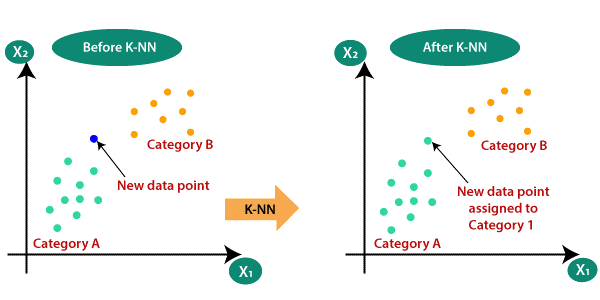
\includegraphics[width=\linewidth]{images/knnexp.png}
        \caption{K-Nearest Neighbors}
        \label{fig:knn}
    \end{figure}
    
    The K-NN algorithm is a supervised machine learning algorithm that can be used to solve both classification and regression tasks. \\

\textbf{How does the k-nearest neighbors algorithm work?} \\

\begin{enumerate}
\item Select the number K of the Neighbors
\item Calculate the Euclidean distance of K number of neighbors
\item Take the K nearest neighbors as per the calculated Euclidean distance.
\item Among these k neighbors, count the number of the data points in each category.
\item Assign the new data points to that category for which the number of the neighbour is maximum.
\end{enumerate}

Suppose we have a new data point and we need to put it in the required category.
\begin{figure}[H]
        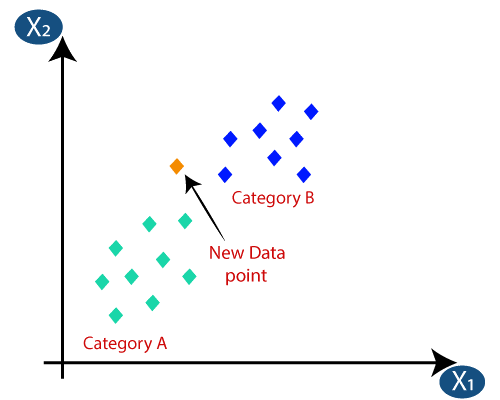
\includegraphics[width=\linewidth]{images/knnexp2.png}
        \caption{K-Nearest Neighbors Datapoint Graph}
        \label{fig:knndp}
\end{figure}
 
\begin{itemize}
\item Firstly, we will choose the number of neighbors, so we will choose the k=5.
\item Next, we will calculate the Euclidean distance (which we learnt in high school) between the data points. The Euclidean distance is the distance between two points, which we have already studied in geometry. It can be calculated as:
\end{itemize}
\begin{equation}
    {D_{Euclidean}} = \sqrt{(x_1-x_2)^2 + (y_1-y_2)^2}
\end{equation}

\begin{figure}[H]
    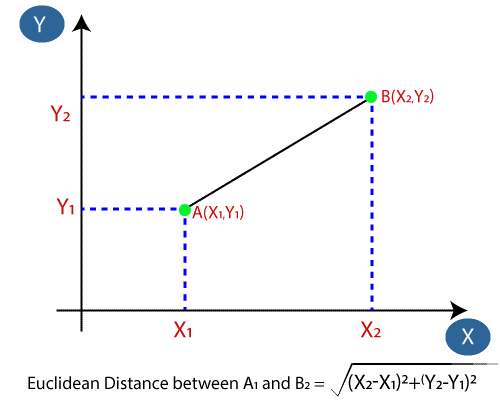
\includegraphics[width=\linewidth]{images/knnexp3.png}
    \caption{Calculating Euclidean distance between two data points}
    \label{fig:exp3}
\end{figure}

By calculating the Euclidean distance, we got the nearest neighbors, as three nearest neighbors in category A and two nearest neighbors in category B. Consider the below image:
\begin{figure}[H]
    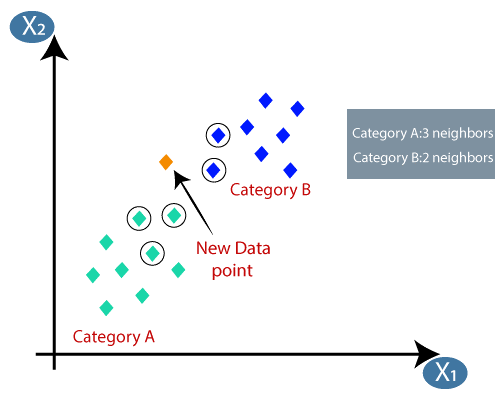
\includegraphics[width=\linewidth]{images/knnexp4.png}
    \caption{Nearest Neighbors}
    \label{fig:knnexp4}
\end{figure}

As we can see the 3 nearest neighbors are from category A, hence this new data point must belong to category A. \\

\textbf{Advantages of KNN Algorithm} \\
\begin{itemize}
\item It is simple to implement.
\item It is robust to the noisy training data
\item It can be more effective if the training data is large.
\end{itemize}

\textbf{Disadvantages of KNN Algorithm} \\
\begin{itemize}
\item Always needs to determine the value of K which may be complex some time.
\item The computation cost is high because of calculating the distance between the data points for all the training samples.
\end{itemize}

\textbf{Distance functions} \\ 

For KNN we can use different distance functions to achieve better accuracy or different K values.

% Euclidean Formula
\begin{equation}
    {D_{Euclidean}} = \sqrt{(x_1-x_2)^2 + (y_1-y_2)^2}
\end{equation}

%Manhattan  Formula
\begin{equation}
    {D_{Manhattan}} = |x_1-x_2| + |y_1-y_2|
\end{equation}

%Minkowski Formula
\begin{equation}
    {D_{Minkowski}} = \left\{ \left[ \left( \left( x_1-x_2 \right)^p \right)^q \right]^r \right\}^{1/r}
\end{equation}

\subsection{Measuring of Performance of Models}

We can use functions in our machine learning libraries to measure performance of our model.

    \begin{figure}[H]
        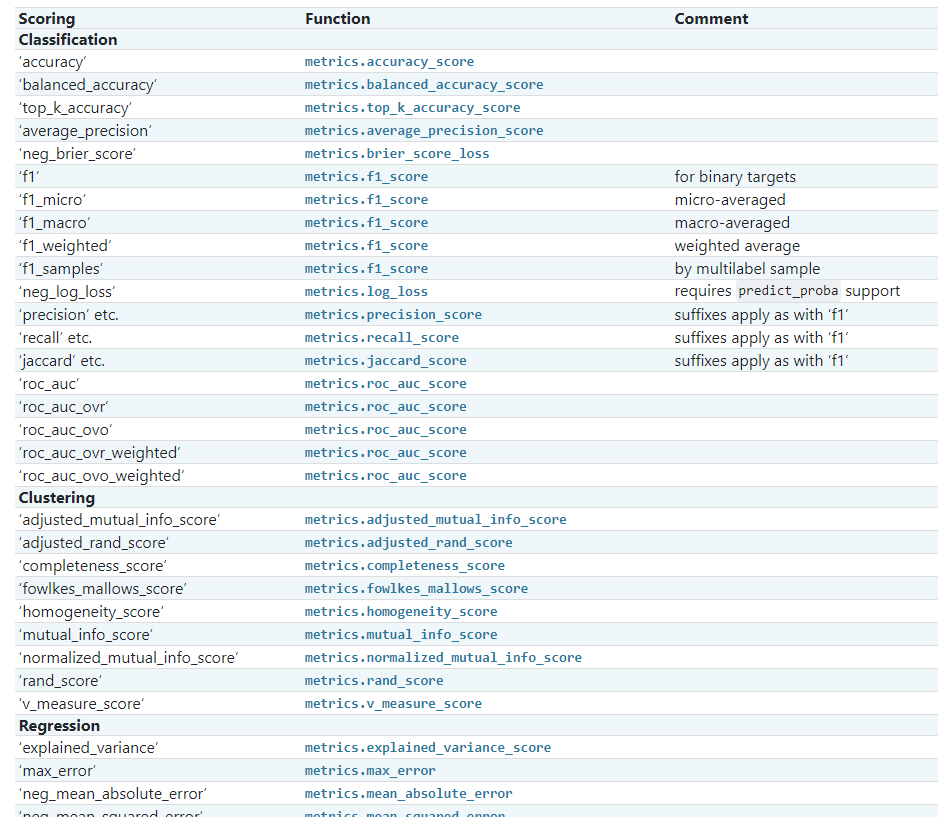
\includegraphics[width=\linewidth]{images/performance.png}
        \caption{Performance measurement functions in Python Scikit-Learn Module}
        \label{fig:perf}
    \end{figure}

above is a photo of performance metrics functions for the module scikit-learn in Python if you research these function names you can view formulas on these tools.

Check out the following link for more information on performance metrics:

\url{https://scikit-learn.org/stable/modules/model_evaluation.html}

\subsubsection{Real life example of model evaluation}

Below is performance metrics on a model I improved on a project of Galaxy Machine Learning.

\begin{figure}[H]
    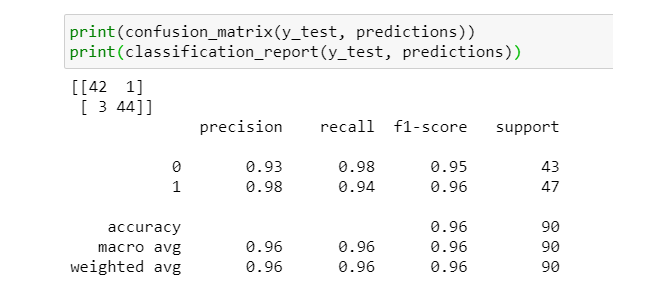
\includegraphics[width=\linewidth]{images/performancemetrics.png}
    \caption{Performance metrics on a model}
    \label{fig:perfex}
\end{figure}

For the model above you can see it has extremely good accuracy of around 96\% accuracy
Anything above 90\% I consider good enough there was times I even got 100\% accuracy for a model. \\
Let’s check out how our F1-Score is calculated. \\

\begin{equation}
    F1\textnormal{-}Score = \frac{2 \times Precision \times Recall}{Precision + Recall}
\end{equation}

alternatively, we can use the following formula:

    \begin{equation}
        F1\textnormal{-}Score = \frac{2TP}{2TP+FP+FN}
    \end{equation}

where TP is the number of true positives, FP is the number of false positives, FN is the number of false negatives. \\

\textbf{What does TP mean?} \\
That means True Positives in our dataset. Which our correct data in our dataset which tested true in our data. \\
\textbf{What does FP mean?} \\
That means False Positives in our dataset. Which our incorrect data in our dataset which tested false in our data. \\
\textbf{What does FN mean?} \\
That means False Negatives in our dataset. Which our incorrect data in our dataset which tested true in our data. \\






Another tool we can use to showcase our TP, FP, FN is called a \textbf{confusion matrix}

Mathematically, a confusion matrix looks like this:

\begin{equation}
    \begin{bmatrix}
        TP & FP \\
        FN & TN
    \end{bmatrix}
\end{equation} \\

Graphically could look like this below
\begin{figure}[H]
    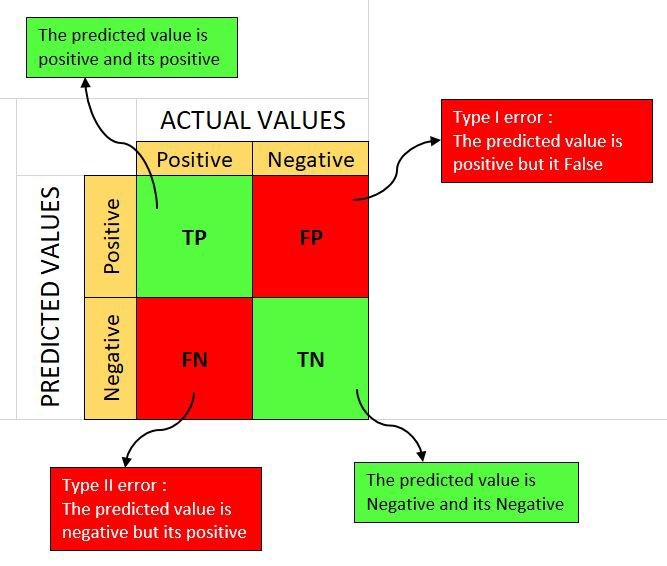
\includegraphics[width=\linewidth]{images/confusionmatrix.jpg}
    \caption{Confusion Matrix}
    \label{fig:confusion}
\end{figure}

Another graphical representation using the ADGMLCLASS library is shown below:
\begin{figure}[H]
    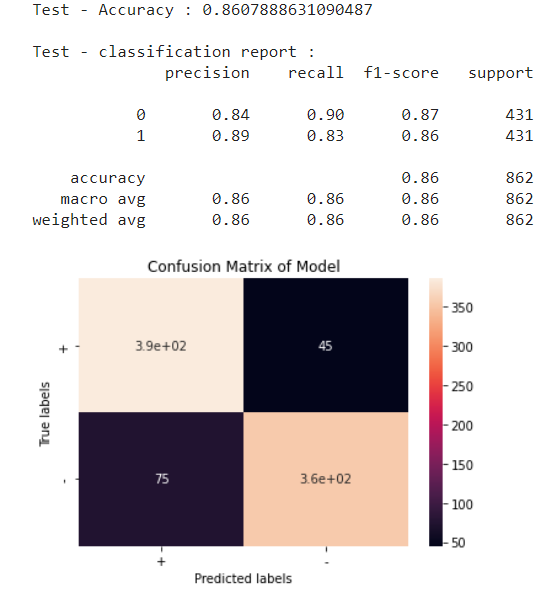
\includegraphics[width=\linewidth]{images/confusionmatrixpt2.png}
    \caption{Real life Confusion Matrix of a model}
    \label{fig:confusion2}
\end{figure}

\subsection{Playing with Machine Learning Demos + Real World Examples I did}

\subsubsection{GalaxyML}

You can play with GalaxyML. I helped a masters student optimize the ML Solution using adgmlclass and put the repo because this is a real-world example of ML in action.  

\begin{figure}[H]
    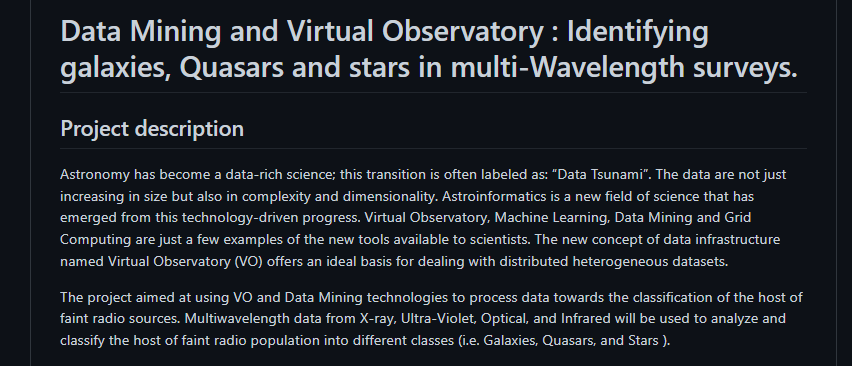
\includegraphics[width=\linewidth]{images/galaxymlrepo.png}
    \caption{GalaxyML Repo}
    \label{fig:galaxyml}
\end{figure}

\begin{center}
    \url{https://github.com/ADGSTUDIOS/GalaxyML}
\end{center}

\subsubsection{Neural Networks}
\begin{figure}[H]
    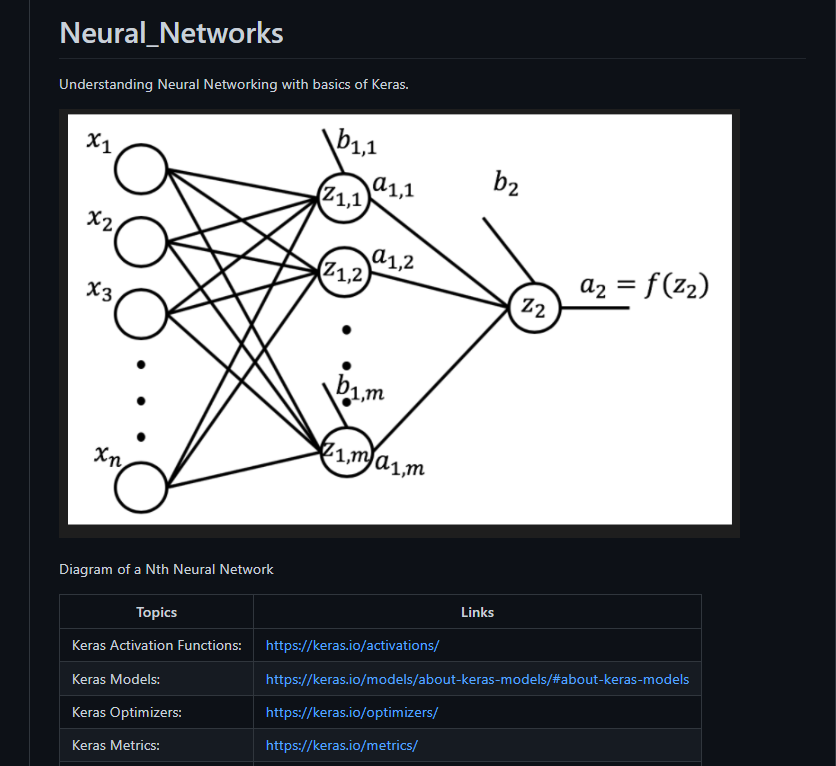
\includegraphics[width=\linewidth]{images/neuralnetworksrepo.png}
    \caption{Neural Networks Repo}
    \label{fig:neuralnetworks}
\end{figure}

If you want to play with Neural Networks got great notebooks to play with @ 
\url{https://github.com/adgsenpai/Neural_Networks}

\subsubsection{Machine Learning Application in ECommerce}

Clothing Size Guide AI Application used for predicting clothing size \\
given a users BUST(CM) and HIPS(CM) \\ 

\begin{figure}[H]
    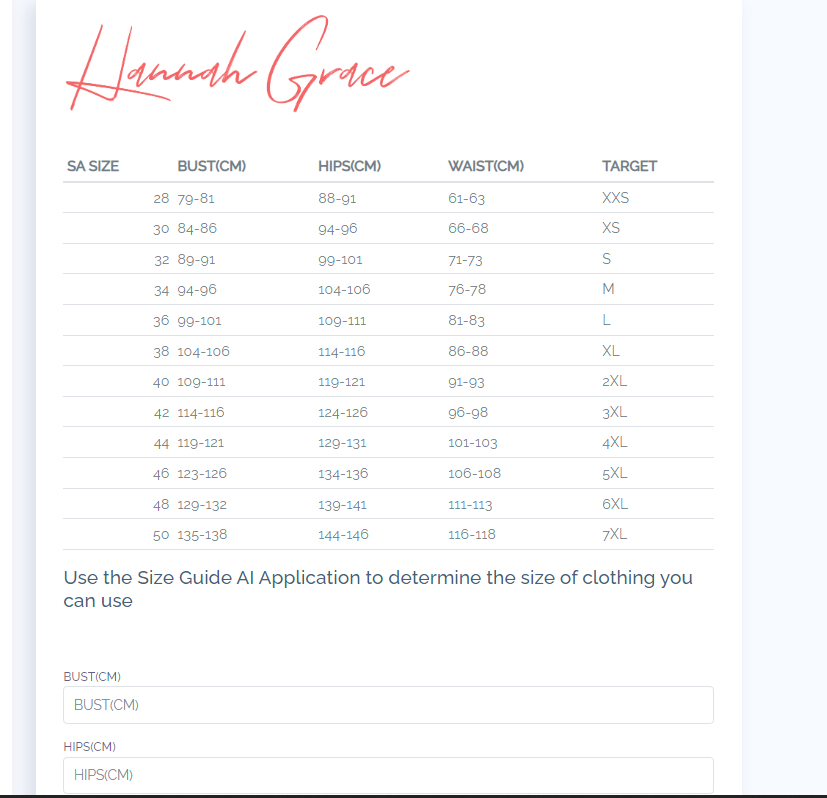
\includegraphics[width=\linewidth]{images/hannahgrace.png}
    \caption{Hannah Grace Clothing Size AI Application}
    \label{fig:clothingai}
\end{figure}

you can play with it @ \url{https://www.hannahgrace.co.za/size-guide/} this app has an accuracy of 100\%

\subsection{Forecasting with Prophet}
\subsubsection{What is Forecasting?}

\textit{Forecasting} is the process of predicting the future based on historical and current data. These can then be compared (resolved) to what actually happens. For example, a company might forecast revenue for the coming year and then compare it to actual results. Prediction is a related but broader term. Forecasting can refer to formal statistical methods that use \textit{time series}, cross-sectional, or longitudinal data, as well as less formal judgmental methods or the prediction and resolution process itself. In hydrology, for example, the terms "forecast" and "forecasting" are sometimes used to refer to estimates of values at specific future times, whereas the term "prediction" is used to refer to more general estimates.
We can use forecasting in digital twins, businesses and the stock market. We will run time series analysis on the data to build a digital twin of any plant or simulation.
A time series analysis is a method of analysing a collection of data points over a period of time. Instead of recording data points intermittently or randomly, time series analysts record data points at consistent intervals over a set period of time. If you refer back to Linear Regression, we will build a forecasting model equation to sketch a time series analysis forecasting graph based on concepts of \textit{Linear Regression}.


\begin{figure}[H]
    \begin{center}
    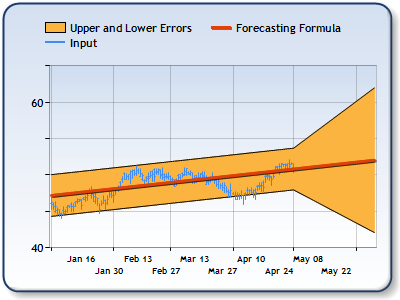
\includegraphics[width=200px]{images/timeseries.png}
    \end{center}
    \caption{Time Series Graph}
    \label{fig:timeseries}
\end{figure}

\subsubsection{What is Prophet?}
\textit{Prophet} is a module for forecasting time series data based on an additive model where non-linear trends are fit with yearly, weekly, and daily seasonality, plus holiday effects. It works best with time series that have strong seasonal effects and several seasons of historical data. Prophet is robust to missing data and shifts in the trend, and typically handles outliers well.
In 2017, Facebook (now called Meta) released Prophet, an open-source forecasting tool in Python and R. The demand for high-quality forecasts often outpaces the analysts producing them. This situation was the motivation behind building a tool like Prophet that makes it easier for both experts and non-experts to deliver high-quality forecasts. Prophet has gained massive popularity among other forecasting tools. Prophet also tops among other Python time series packages when ranked by monthly downloads. It is supported in the Python and R language.
Producing high-quality forecasts is a challenge. Businesses usually resort to either of the two options to create forecasts — they use completely automatic forecasting techniques or are entirely dependent on human analysts to produce high-quality forecasts. Both the options have their own drawbacks. In the case of complete automation, forecasting techniques produced are brittle and inflexible; incorporating useful assumptions becomes difficult. On the other hand, it is a challenge to find analysts who can create forecasts because it requires people with specialized data science skills with substantial experience. To remediate these challenges, Prophet attempts to offer the best of both worlds. Users are not left at the complete mercy of an automatic process; instead, an analyst with no training in time series can help improve and tweak forecasts using easily interpretable parameters. According to Meta, Prophet offers a straightforward way to create a ‘reasonable and accurate forecast’. Further, the forecasts made by Prophet are customisable in a way that is intuitive to even non-experts.


\subsubsection{How does Prophet work mathematically? + Prophet models explained mathematically.}
The Prophet procedure is an additive regression model with four main components — a piecewise linear logistic growth curve trend; a yearly seasonal component modelled using Fourier series; a weekly seasonal component created using dummy variables; a user-provided list of important holidays. The procedure makes use of a decomposable time series model with three main model components: trend, seasonality, and holidays. This is an important technique for all types of time series analysis, especially for seasonal adjustment. It seeks to construct, from an observed time series, a number of component series (that could be used to reconstruct the original by additions or multiplications) where each of these has a certain characteristic or type of behaviour.
Similar to a generalized additive model (GAM), with time as a regressor.
In statistics, a generalized additive model (GAM) is a generalized linear model in which the linear response variable depends linearly on unknown smooth functions of some predictor variables, and interest focuses on inference about these smooth functions.
Prophet fits several linear and non-linear functions of time as components. In its simplest form;

\begin{equation}
    y(t) = g(t) + s(t) + h(t) + e(t)
\end{equation} \\ 
    
$g(t)$ - trend models non-periodic changes (i.e., growth over time) \\ 
$s(t)$ - seasonality presents periodic changes (i.e., weekly, monthly, yearly) \\ 
$h(t)$ - ties in effects of holidays (on potentially irregular schedules $\geq$ 1 day(s)) \\
$e(t)$ - covers idiosyncratic changes not accommodated by the model \\ 

In other words, the procedure’s equation can be written;

\begin{equation}
    y(t)=piecewise_{trend}(t) +seasonality(t)+holiday_{effects}(t) +noise(t)
\end{equation} \\

\subsubsection{Trends}
The procedure provides two possible trend models for $g(t)$, “a saturating growth model, and a piecewise linear model.”

\subsubsection{Saturating Growth Model}
If the data suggests promise of saturation — i.e., one is wrestling constraints like: Power station capacity levels gigawatts (GW), Water Production Capacity (Megalitre), — 
setting growth= $"logistic"$ is the move.
Typical modelling of these nonlinear, saturating trends is basically accomplished;

\begin{equation}
    g(t) = \frac{1}{1+e^{-\frac{t-t_0}{\tau}}}
\end{equation} \\
    
    where $t_0$ is the time of the first data point, $tau$ is the time constant, and $t$ is the time. \\

alternatively in Prophet \\ 
\begin{equation}
    g(t) = \frac{1}{1+e^{-k(t-m)}}
\end{equation} \\
    
where:
$C$ is the carrying capacity
$k$ is the growth rate
$m$ is an offset parameter
There are two primary aspects of growth at Facebook (fluctuating carrying capacity and volatile rate of change) that are not captured in this simplified equation, though. \\

\textbf{Carrying Capacity vs Time} \\ 

First, as with many scalable business models carrying capacity is not constant — as “the population increases the capacity demands scale for plants the plants need to cater for the ever-growing population”, so does the growth ceiling.”
Accounting for this is done by replacing the fixed capacity C with a time-varying capacity C(t). \\

\textbf{Rate of Change vs Time} \\
Second, the market does not allow for stagnant technology. Advances like those seen over the past decade in handheld devices, app development, and global connectivity, virtually ensure that growth rate is not constant.
Because this rate can quickly compound due to new products, the model must be able to incorporate a varying rate in order to fit historical data. \\

Suppose there are S changepoints at times $\delta{j},j = 1,...,S $ \\

Prophet defines a vector of rate adjustments;
\begin{equation}
    \delta{j} \in \mathbb{R}^S
\end{equation} \\

where:
$\delta{j}$ is the rate adjustment for the $j$th changepoint
$S$ is the number of changepoints

The rate at any time t is then the base rate k, plus adjustments up to that time;
\begin{equation}
    k(t) = k + \sum_{j=1}^{S} \delta{j} \left\{ \frac{t-\delta{j}}{1+\delta{j}} \right\}
\end{equation} \\

This is represented more cleanly by defining a vector;
\begin{equation}
    a(t) \in \{0,1\} ^S
\end{equation} \\

Described by Meta \\
“The rate at time t is then $k+a(t)^T\delta$ When the rate $k$ is adjusted, the offset parameter $m$ must also be adjusted to connect the endpoints of the segments. The correct adjustment at changepoint $j$ is easily computed as”
\begin{equation}
    \delta{j} = \frac{m-\delta{j-1}}{1+\delta{j-1}}
\end{equation} \\

At last, the piecewise growth= $"logistic"$ model is reached;
\begin{equation}
    g(t) = \frac{1}{1+e^{-k(t-m)}}
\end{equation} \\

In application, the logistic growth model presented here is a special case of generalized logistic growth curves — which is only a single type of sigmoid curve — allowing the relatively straightforward extension(s) of this trend model to other families of curves.

\subsubsection{Linear Trend with Changepoints}

The second — much simpler and default — trend model is a simple Piecewise Linear Model with a constant rate of growth. It is best suited for problems without a market cap or other max in sight, and is set via $growth='linear'$.
Modelling the linear trend is easily realized with Prophet. In fact, not adjusting anything usually does the trick;

\begin{equation}
    g(t)= (k+a(t)^T \delta  )t+(m+a(t)^T \gamma )
\end{equation} \\

where:
$k$ is the growth rate
$\delta $ has the rate adjustments
$m$ is the offset parameter

and, to make the function continuous, $\gamma j$ is set to:
\begin{equation}
    \gamma j = \frac{m-\gamma j-1}{1+\gamma j-1}
\end{equation}

I think in Metas case could be interpreted as:
\begin{equation}
    -s_j \delta_j
\end{equation} \\

\subsubsection{Automatic Changepoint Selection}
If known, the changepoints $s_j$ can be specified by the user as dates of product launches and other growth-altering events (one example in the plants, measurements in the labs at a specific date), or, by default, changepoints may be automatically selected given a set of candidates.\\
“Automatic selection can be done quite naturally with the formulation in either model by putting a sparse prior on $\delta$.” - Meta \\ 
Often, it is advisable to specify a large number of changepoints (e.g., one per month for a several years history, in plants we typically have weekly data or daily data that’s a lot of data, I worked with a dataset of 1 million samples of a plant) and use the prior:
\begin{equation}
    \delta{j} \sim \mathcal{L}(0,\tau)
\end{equation} \\

where: \\
$\tau$ directly controls the flexibility of the model in altering its rate.

Critical note: a sparse prior on the adjustments $\delta$ has no impact on the primary growth rate k, so as $\tau$ progresses to 0 the fit reduces to standard (not-piecewise) logistic or linear growth.

\subsubsection{Trend Forecast Uncertainty}
When the model is extrapolated past the history to make a forecast, the trend $g(t)$ will have a constant rate; the uncertainty in the forecast trend is estimated by extending the generative model forward.\\

The generative model for the trend is that there are; \\ 
\begin{itemize}
\item	S changepoints
\item	over a history of T points
\item	each of which has a rate change $\delta{j} \sim \mathcal{L}(0,\tau)$
\end{itemize}

Simulation of future rate changes (that emulate those of the past) is achieved by replacing $\tau$ with a variance inferred from data. \\

“In a fully Bayesian framework this could be done with a hierarchical prior on $\tau$ to obtain its posterior, otherwise we can use the maximum likelihood estimate of the rate scale parameter” - Meta

\begin{equation}
    \lambda = \frac{1}{S} \sum_{j=1}^{S} | \delta_{j} |
\end{equation}

“Future changepoints are randomly sampled in such a way that the average frequency of changepoints matches that in the history”
- Meta

\begin{equation}
    \forall{j} > T ,
    \left\{
        \begin{array}{lr}
            \delta_{j} = 0 & w.p. \frac{T-S}{T} \\
            \delta_{j} \sim \mathcal{L}(0,\tau) & w.p. \frac{S}{T}        
        \end{array}
    \right\} 
\end{equation} \\

Thus, uncertainty in the forecast trend is measured by assuming the future will see the same average frequency and magnitude of rate changes that were seen in the history. Once $\lambda $ has been inferred from the data, this generative model is deployed to “simulate possible future trends and use the simulated trends to compute uncertainty intervals.” Prophet’s assumption that the trend will continue to change with the same frequency and magnitude as it has in the history is fairly strong, so don’t bank on the uncertainty intervals having exact coverage.
As $\tau $ is increased the model has more flexibility in fitting the history and so training error will drop. Even so, when projected forward this flexibility is prone to produce wide intervals. The uncertainty intervals are, however, a useful indication of the level of uncertainty, and especially an indicator of over fitting.

\subsubsection{Seasonality}

The seasonal component $s(t)$ provides an adaptability to the model by allowing periodic changes based on sub-daily, daily, weekly and yearly seasonality.
“Business time series often have multi-period seasonality as a result of the human behaviours they represent. For instance, a 5-day work week can produce effects on a time series that repeat each week, while vacation schedules and school breaks can produce effects that repeat each year. To fit and forecast these effects we must specify seasonality models that are periodic functions of $t$.”
Prophet relies on Fourier series to provide a malleable model of periodic effects. $P$ is the regular period the time series will have (e.g., $P$ = 365.25 for yearly data or $P$ = 7 for weekly data, when time is scaled in days).
Approximate arbitrary smooth seasonal effects are therefore tied in with a standard Fourier series;

\begin{equation}
    s(t) = \sum_{n=1}^{N} {a_n} \cos \left( \frac{2\pi n}{P} t \right) + \sum_{n=1}^{N} b_n \sin \left( \frac{2\pi n}{P} t \right)
\end{equation}

“Fitting seasonality requires estimating the $2N$ parameters $\beta =[a1,b1,…,aN,bN]^T$. This is done by constructing a matrix of seasonality vectors for each value of t in our historical and future data, for example with yearly seasonality and $N$= 10” - Meta

\begin{equation}
    X(t) = (\cos(\frac{2\pi (10)t}{365.25}),...,\sin(\frac{2\pi (10)t}{365.25}) )
\end{equation} \\

Meaning the seasonal component is;
\begin{equation}
    s(t)=X(t)\beta 
\end{equation}

In the generative model, Prophet takes $\beta \sim Normal(0,\sigma^2)$ to impose a smoothing prior on the seasonality.
Truncating the series at N applies a low-pass filter to the seasonality, so, albeit with increased risk of overfitting, increasing N allows for fitting seasonal patterns that change more quickly.
“For yearly and weekly seasonality, we have found N = 10 and N = 3 respectively to work well for most problems. The choice of these parameters could be automated using a model selection procedure such as AIC.” ~ Meta

\subsubsection{Holidays and Events}

Impact of a particular holiday on the time series is often similar year after year, making it an important incorporation into the forecast. The component $h(t)$ speaks for predictable events of the year including those on irregular schedules. To utilize this feature, the user needs to provide a custom list of events. Fusing this list of holidays into the model is made straightforward by assuming that the effects of holidays are independent.\\


\begin{tabular}{ |p{6cm}||p{6cm}|}
    \hline
    \multicolumn{2}{|c|}{South African Public Holidays in the year 2022} \\
    \hline
    Holiday name & Date\\
    \hline
    New Year’s Day &	Sat, 01 Jan 2022\\
    Human Rights Day &	Mon, 21 Mar 2022\\
    Good Friday &	Fri, 15 Apr 2022\\
    Family Day &	Mon, 18 Apr 2022\\
    Freedom Day &	Wed, 27 Apr 2022\\
    Workers’ Day &	Mon, 02 May 2022\\
    Youth Day (in South Africa) &	Thu, 16 Jun 2022\\
    National Women’s Day &	Tue, 09 Aug 2022\\
    Heritage Day & 	Sat, 24 Sept 2022\\
    Day of Reconciliation &	Fri, 16 Dec 2022\\
    Boxing Day &	Mon, 26 Dec 2022\\
    Christmas Day &	Likely Mon, 26 Dec 2022    \\
    \hline
\end{tabular} \\ 

We could define a function called public holidays and generate a list of public holidays. We can implement an API maybe also to get the holidays with dates in any country at a given time interval. In layman’s terms our equation and data structure (as a dictionary mathematically a set) will be described as below:
\begin{align*}
holidayAPI({countryName,year})&=\{i_0 HolidayName:i_0 HolidayDate \\
&,i_1 HolidayName:i_1HolidayDate,…\\
&,i_{lastindex} HolidayName:i_{lastindex} HolidayDate\}
\end{align*}\\

Our API can be described like that above returning all the holidays for a given year. Once we got an algorithm like that going.

\begin{equation} 
    h(t) = \sum_{t=startDate}^{endDate} \{ holidayAPI\{countryName,t\} \} 
\end{equation}

We could define a function called public holidays and generate a list of public holidays. We can implement an API maybe also to get the holidays with dates in any country at a given time interval. In layman’s terms our equation and data structure (as a dictionary mathematically a set) will be described as below:

We finalize the algorithm to get all the holidays during a time interval. But in machine learning we don’t really need to know the holiday name so formally how we work this data mathematically is shown below formally we just use the past and future dates of the holiday.
For each holiday $i$, let $D_i$ be the set of past and future dates for that holiday. Then add an indicator function representing whether time t is during holiday $i$, and assign each holiday a parameter $K_i$ which is the corresponding change in the forecast.\\

This is done in a similar way as seasonality by generating a matrix of regressors; \\
\begin{equation}
    Z(t)= [1(t \in D_1),…,1(t \in D_L)]] 
\end{equation} \\

and taking,

\begin{equation}
    h(t) = Z(t)\kappa 
\end{equation} \\

As with seasonality, Prophet uses a prior $\kappa-Normal(0,v^2)$. \\ 

“It is often important to include effects for a window of days around a particular holiday, such as the weekend of Thanksgiving. To account for that we include additional parameters for the days surrounding the holiday, essentially treating each of the days in the window around the holiday as a holiday itself.” - Meta

\subsubsection{Prophet Conclusion}
Ultimately, Prophet was engineered to help analysts with a variety of backgrounds produce more forecasts with less time invested towards doing so. This was achieved by sticking to a relatively plain model. \\ 
“We use a simple, modular regression model that often works well with default parameters, and that allows analysts to select the components that are relevant to their forecasting problem and easily make adjustments as needed.” - Meta

\subsubsection{Prophet Resources}
Official Prophet Meta Website \\ 
\url{https://facebook.github.io/prophet/} \\
Official Developer Documentation \\
\url{https://facebook.github.io/prophet/docs/quick_start.html} \\
Blog \\
\url{https://research.facebook.com/blog/2017/02/prophet-forecasting-at-scale/}
Prophet Thesis Paper \\
\url{https://peerj.com/preprints/3190/} \\ 
I am not allowed to disclose my industrial work of a digital twin which I built of a plant but I do have an example which you can use on how I used prophet for building Opportunity Stonks. \\ 

\begin{figure}[H]
    \centering
    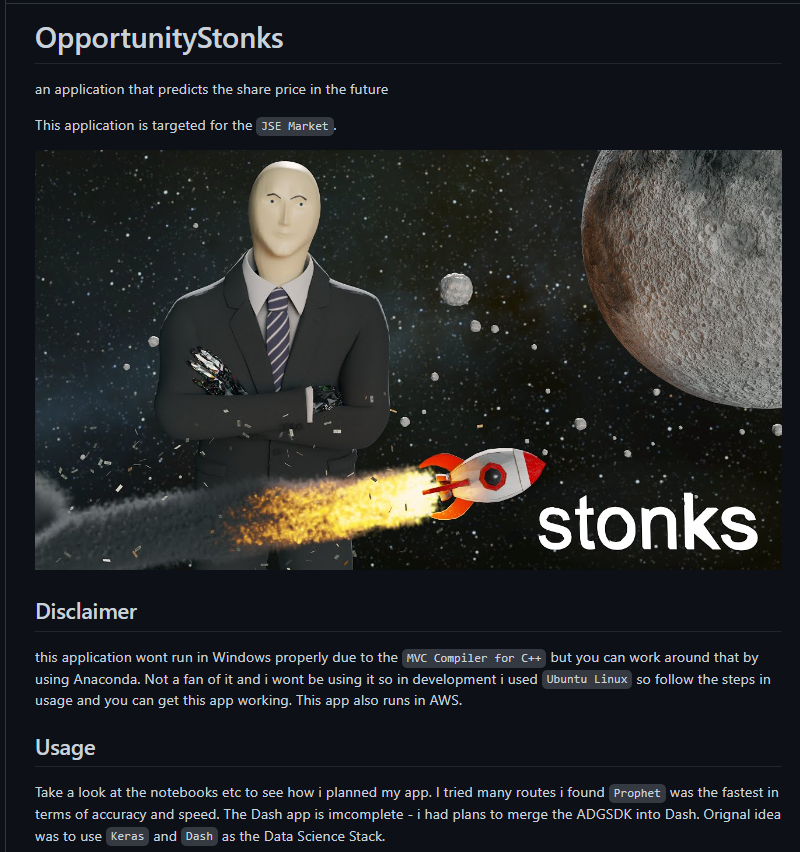
\includegraphics[width=0.8\textwidth]{opportunitystonks.png}
    \caption{GitHub Repo for Opportunity Stonks \url{https://github.com/adgsenpai/OpportunityStonks}}
    \label{fig:opportunitystonks}
\end{figure} 

\begin{figure}[H]
    \centering
    \includegraphics[width=0.8\textwidth]{stonkapppt1.png}
    \caption{Screenshot of Opportunity Stonks}
    \label{fig:opportunitystonks2}
\end{figure} 

\begin{figure}[H]
    \centering
    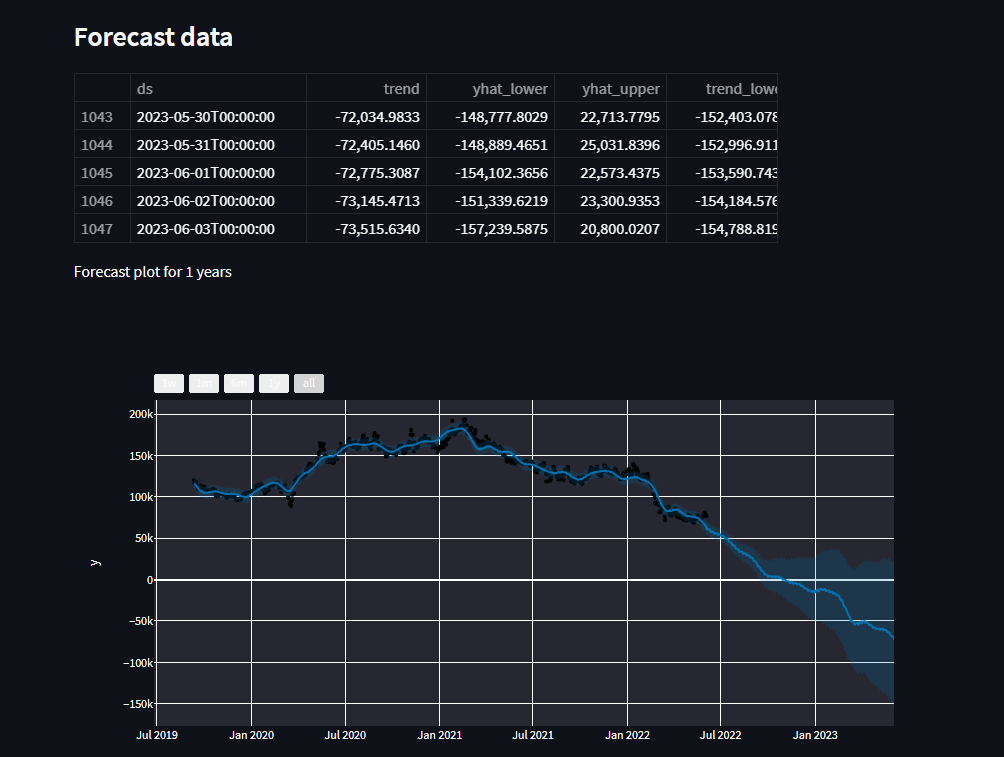
\includegraphics[width=0.8\textwidth]{stonkapppt2.png}
    \caption{Time Series Analysis/Forecast of Stock using Prophet @ Opportunity Stonks}
    \label{fig:opportunitystonks3}
\end{figure}

\section{Building Digital Twins}

\subsection{Revising Methodology to Build Digital Twins}

The first step to building digital twins is that you need to collect your data depending on the type of digital twin you are building. \\

Examples: \\

\begin{itemize}
\item    If you are building a digital twin of a plant – you will need to get $n$th number of records over a $t$ period of that plant. You can be at the plant taking measurements or asking permission at a company for the datasets.
\item	If you are building a general digital twin of anything for fun or research. You can get a dataset publicly from the internet. A good start to any data science project is playing around with datasets implementing algorithms and demo apps to get a grip on projects.
        A good website for datasets is \url{https://www.kaggle.com/datasets}
\end{itemize}    

\begin{figure}[H]
    \centering
    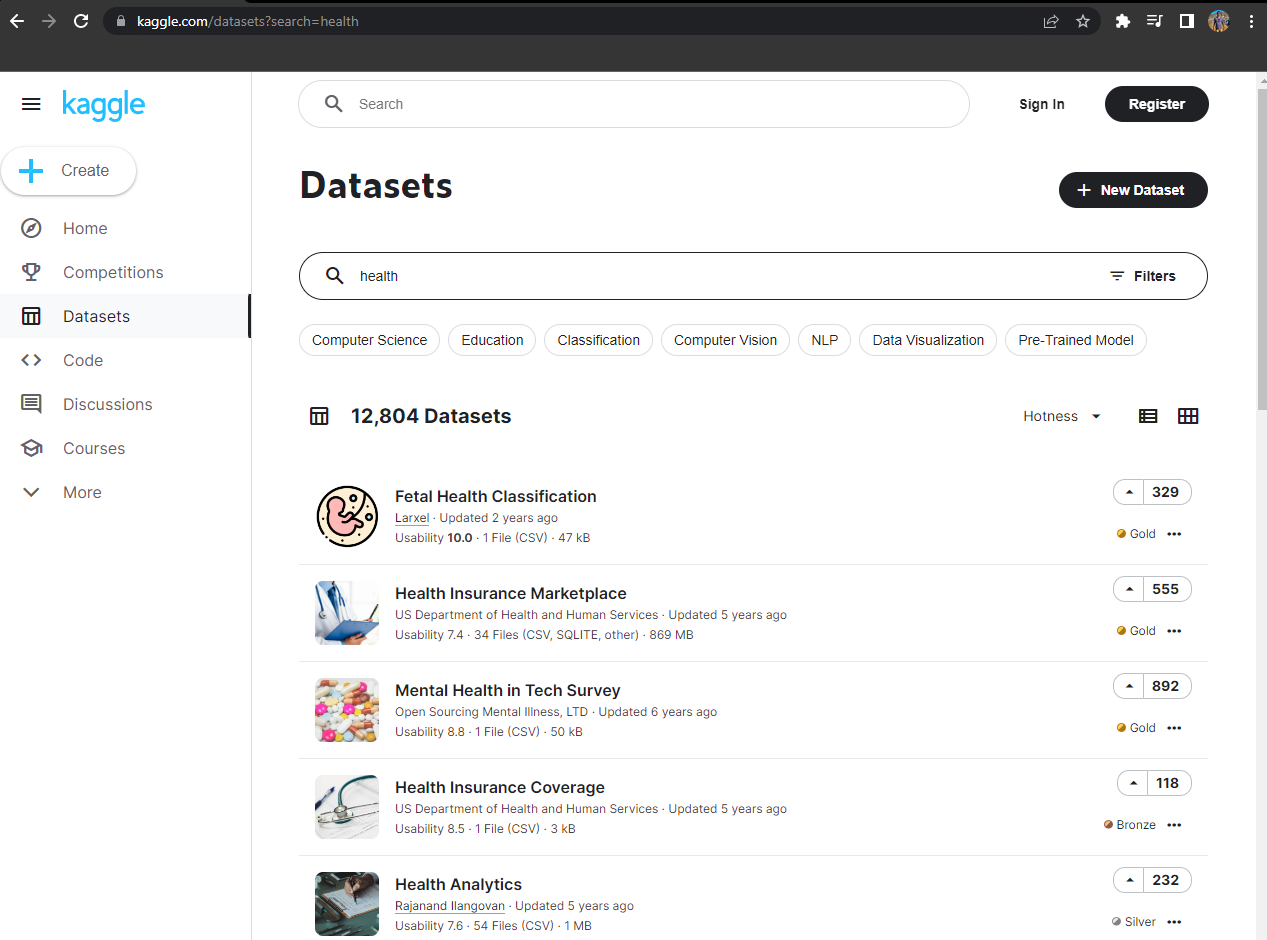
\includegraphics[width=0.8\textwidth]{kaggle.png}
    \caption{
        Kaggle Website for datasets - query for "Health"
        }
    \label{fig:dataset}
\end{figure}

The second step is that you must visualize your dataset, Learn about your parameters/variables. You can do that by sketching graphs it can be different types of graphs but different graphs might work better to visualize that relationship.
The third step is that you must try different algorithms and play around with Machine Learning tools and Time Series Analysis Tools. Make sure your data is clean! 
The final step is that you can combine steps 2 and 3 into a cool looking dashboard for companies to play with on the web. Why the web? Because it is cross-platform.

\subsection{Python Modules that can help you out when building digital twins}

\textbf{Pandas} - Pandas is a software library written for the Python programming language for data manipulation and analysis. In particular, it offers data structures and operations for manipulating numerical tables and time series. It is free software released under the three-clause BSD license. We normally use that for .xlsx files, .csv, .sql databases and etc.\\
\textbf{Prophet} – Forecasting, Time Series Analysis Module by Meta, as discussed above in the paper\\
\textbf{Streamlit} - Streamlit is an open-source app framework in Python language. It helps us create web apps for data science and machine learning in a short time. It is compatible with major Python libraries such as scikit-learn, Keras, PyTorch, SymPy(latex), NumPy, pandas, Matplotlib etc.\\
\textbf{Keras} - Keras is an open-source software library that provides a Python interface for artificial neural networks. Keras acts as an interface for the TensorFlow library. Up until version 2.3, Keras supported multiple backends, including TensorFlow, Microsoft Cognitive Toolkit, Theano, and PlaidML.\\
\textbf{Tensorflow} - TensorFlow is a free and open-source software library for machine learning and artificial intelligence. It can be used across a range of tasks but has a particular focus on training and inference of deep neural networks.\\
\textbf{Dash} - Dash is a Python module or framework used to create many analytical web applications, and we can build analytical dashboards using a dash framework. With the help of the Dash module, we can easily create very fast and responsive web dashboards, which are also very good to look at (Having a Great User Interface).\\
\textbf{Numpy} - NumPy is a library for the Python programming language, adding support for large, multi-dimensional arrays and matrices, along with a large collection of high-level mathematical functions to operate on these arrays.\\
\textbf{SciPy} - SciPy is a free and open-source Python library used for scientific computing and technical computing. SciPy contains modules for optimization, linear algebra, integration, interpolation, special functions, FFT, signal and image processing, ODE solvers and other tasks common in science and engineering.\\
\textbf{Seaborn} - Seaborn is an open-source Python library built on top of matplotlib. It is used for data visualization and exploratory data analysis. Seaborn works easily with dataframe and
the Pandas library. The graphs created can also be customized easily\\
\textbf{matplotlib.pyplot} - is a collection of functions that make matplotlib work like MATLAB. Each pyplot function makes some change to a figure: e.g., creates a figure, creates a plotting area in a figure, plots some lines in a plotting area, decorates the plot with labels, etc.








 



















